\newcommand{\FS}{
  \begin{figure}
    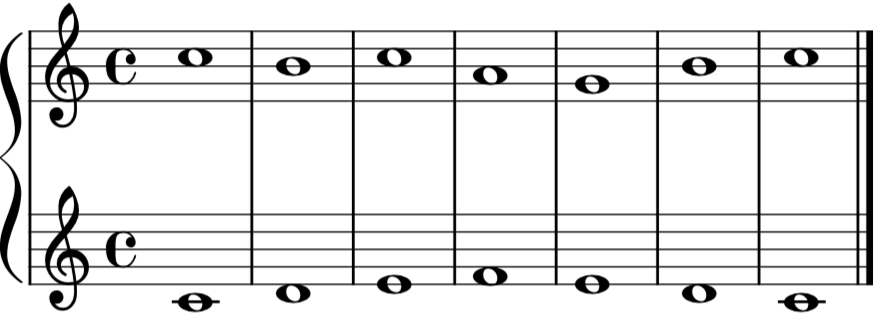
\includegraphics[width=6cm]{fig/fs.png}
    \caption{First Species Counterpoint}
    \label{fig:fs}
  \end{figure}
}

\newcommand{\Motion}{
  \begin{figure}
    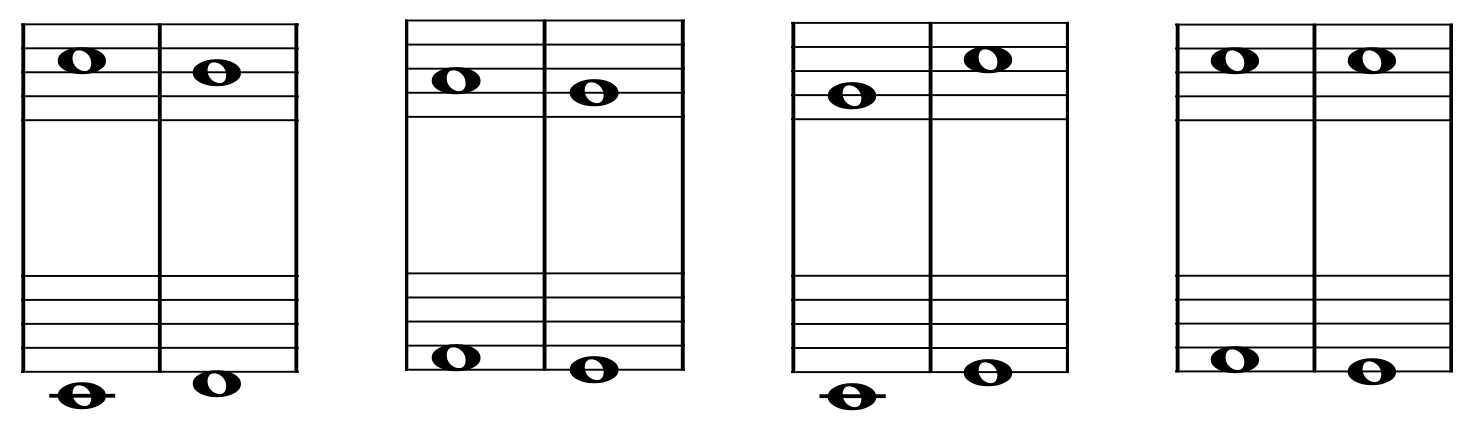
\includegraphics[width=6cm]{fig/motion.png}
    \hspace{1cm}
    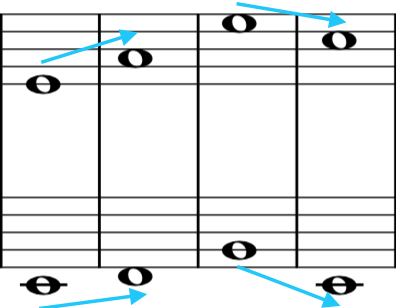
\includegraphics[width=3cm]{fig/badmotion.png} \\
    \begin{flushleft}
    \begin{small}
      \hspace{1.95cm} contrary \ \ \ \ parallel \ \ \ \ \ \ \ similar \ \ \ \ \ \ oblique
      \hspace{2.2cm} 5th \hspace{9.5mm} 8th
    \end{small}
    \end{flushleft}
    \caption{Left: Four Kinds of Motion, Right: Invalid Motion}
    \label{fig:motion}
  \end{figure}
}

\renewcommand{\SS}{
  \begin{figure}
    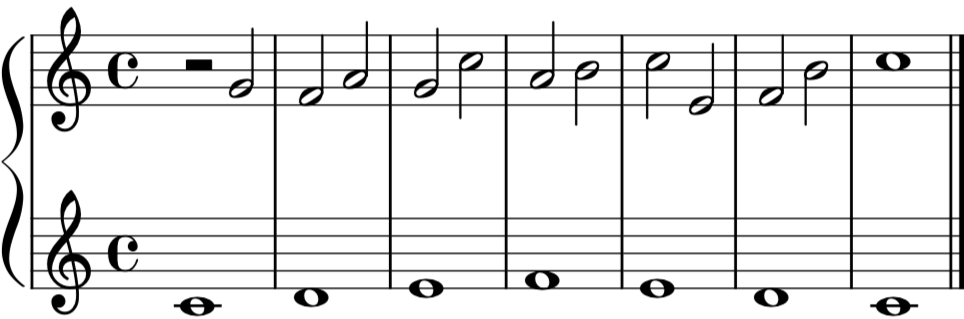
\includegraphics[width=7cm]{fig/ss.png}
    \caption{Second Species Counterpoint}
    \label{fig:ss}
  \end{figure}
}

\section{Counterpoint}
\label{sec:cp}

Counterpoint is a technique for combining multiple lines of melodies.
Composing counterpoint is like arranging a song for choir:
we start with a \emph{cantus firmus}, which serves as the base melody,
and compose counterpoint lines above or below the cantus firmus.
When doing this, we must make sure that the whole music sounds
harmonically pleasing, and that the individual melodic lines are
distinguishable to the listener.

In this section, we present an implementation of species counterpoint,
based on the formulation given by Fux~\citep{fux-cp}.
The idea is to represent ``good'' counterpoint  as a dependent record,
whose fields encode the musical content as well as proofs that the
counterpoint follows certain rules.
For space reason, we only describe two variants of species counterpoint;
other variants can be formalized in an analogous way.

\subsection{First Species Counterpoint}
\label{sec:cp:fs}

\FS

First species counterpoint is the simplest variant of counterpoint.
In first species, we set one note against each note in the cantus firmus,
which is required to start with a tonic and consist only of whole notes.
Figure~\ref{fig:fs} shows an example of first species counterpoint.
The lower line is the cantus firmus, which we excerpt from a famous
German song called ``Froschgesang'' (Frog's song).
The upper line is the counterpoint composed by the second author.

\subsubsection{Representing Music}

In our implementation, we represent each bar as a pitch-interval pair
\texttt{(p ,  i)}, where \texttt{p} is the pitch of a cantus firmus note,
and \texttt{i} is the interval between \texttt{p} and the corresponding
counterpoint note.
We then represent a sequence of bars as a list of pitch-interval pairs,
but with one proviso: we separate the first and last bars from the
middle bars.
Therefore, the Frog's song in Figure~\ref{fig:fs} is represented as a
compound of the following three elements:

\begin{alltt}
 PitchInterval : Set
 PitchInterval = Pitch \(\times\) Interval
  
first : PitchInterval
first = (c 5 , per8)

middle : List PitchInterval
middle = (d 5 , maj6) :: (e 5 , min6) :: (f 5 , maj3) ::
         (e 5 , min3) :: (d 5 , maj6) :: []

last : PitchInterval
last = (c 5 , per8)
\end{alltt}

\subsubsection{Representing Rules}

The reason behind our three-part representation of music is that
different parts are subject to different rules, as we detail below.

\paragraph{Beginning}

The beginning of the music should express perfection.
As we saw in Section~\ref{sec:music}, there are three intervals that
are classified as perfect: the 1st (more commonly called the
\emph{unison}), the 5th, and the 8th.
The first interval of the music must then be one of these intervals.
In our formalization, we implement this rule as the
\texttt{checkBeginning} function, which reports an error
\texttt{not158 i} when the first interval \texttt{i} is an invalid one.
Since Agda does not have exceptions, we turn the error into an option
value by wrapping it around the \texttt{just} constructor.

\begin{alltt}
data BeginningError : Set where
  not158   : PitchInterval \(\rightarrow\) BeginningError
  
checkBeginning : PitchInterval \(\rightarrow\) Maybe BeginningError
checkBeginning pi@(_ , i) =
  if ((i == per1) \(\vee\) (i == per5) \(\vee\) (i == per8))
  then nothing
  else just (not158 pi)
\end{alltt}

\paragraph{Intervals}

The middle bars of the music should maintain harmonical consonance
and independence of melodic lines.
As we saw before, consonant intervals include the unison,
3rd\footnote{We use ``3rd'' to mean both the major and minor variants
of the 3rd interval, and similarly for the 6th.}, 5th, 6th, and 8th,
and among these, the unison is clearly an obstacle to distinguishing
between the two lines of music.
Therefore, the middle bars must consist of the latter four intervals.
We encode this rule as the \texttt{checkIntervals} function, which
returns a list of errors correponding to the occurrences of dissonant
intervals and unisons.

\begin{alltt}
data IntervalError : Set where
  dissonant : Interval \(\rightarrow\) IntervalError
  unison    : Pitch \(\rightarrow\) IntervalError

intervalCheck : PitchInterval \(\rightarrow\) Maybe IntervalError
intervalCheck (p , i) with isConsonant i | isUnison i
... | false | _    = just (dissonant i)
... | _     | true = just (unison p)
... | _     | _    = nothing

checkIntervals : List PitchInterval \(\rightarrow\) List IntervalError
checkIntervals = mapMaybe intervalCheck
\end{alltt}

\paragraph{Motion}

\Motion

The independence of melodic lines is also affected by \emph{motion},
i.e., the way one interval moves to another interval.
As can be seen from Figure~\ref{fig:motion} left, there are four
kinds of motion: \emph{contrary} (two lines go in different directions),
\emph{parallel} (two lines go in the same direction by the same
distance), \emph{similar} (two lines go in the same direction),
and \emph{oblique} (one line plays the same note).
There is a consensus that approaching a perfect interval by parallel
or similar motion (as in Figure~\ref{fig:motion} right) destroys the
independence of lines.
To rule out this, we define the \texttt{checkMotion} function, which
lists all occurrences of such invalid motion.

\begin{alltt}
data MotionError : Set where
  parallel : PitchInterval \(\rightarrow\) PitchInterval \(\rightarrow\) MotionError
  similar  : PitchInterval \(\rightarrow\) PitchInterval \(\rightarrow\) MotionError

motionCheck : PitchInterval \(\rightarrow\) PitchInterval \(\rightarrow\) Maybe MotionError
motionCheck i1 i2 with motion i1 i2 | isPerfect (proj\(\sb{\mathtt{2}}\) i2)
motionCheck i1 i2 | contrary | \_     = nothing
motionCheck i1 i2 | oblique  | \_     = nothing
motionCheck i1 i2 | parallel | false = nothing
motionCheck i1 i2 | parallel | true  = just (parallel i1 i2)
motionCheck i1 i2 | similar  | false = nothing
motionCheck i1 i2 | similar  | true  = just (similar i1 i2)

checkMotion : List PitchInterval \(\rightarrow\) List MotionError
checkMotion = mapMaybe (uncurry motionCheck) \(\circ\) pairs
-- where pairs returns a list of all adjacent pairs in a given list
\end{alltt}

\paragraph{Ending}

The ending of the music should express relaxation.
Among different intervals, the unison and the 8th are considered
most stable, hence the last interval of the music must be either of
these intervals.
The last interval should also be approached by a \emph{cadence},
a progression that gives rise to a sense of resolution.
We encode these rules as the \texttt{checkEnding} function.
Note that it returns the \texttt{tooShort} error when the music does
not have enough number of bars to form a valid ending.

\begin{alltt}
data EndingError : Set where
  not18    : PitchInterval \(\rightarrow\) EndingError
  not27    : PitchInterval \(\rightarrow\) EndingError
  tooShort : List PitchInterval \(\rightarrow\) EndingError

endingCheck : PitchInterval \(\rightarrow\) PitchInterval \(\rightarrow\) Maybe EndingError
endingCheck pi1@(pitch p , i) (pitch q , interval 0)  = 
  if ((p + 1 \(\equiv\sp{\mathtt{b}}\) q) \(\wedge\) (i == min3)) then nothing else just (not27 pi1)
endingCheck pi1@(pitch p , i) (pitch q , interval 12) =
  if ((q + 2 \(\equiv\sp{\mathtt{b}}\) p) \(\wedge\) (i == maj6) \(\vee\) (p + 1 \(\equiv\sp{\mathtt{b}}\) q) \(\wedge\) (i == min10))
  then nothing
  else just (not27 pi1)
endingCheck pi1               pi2                     =
  just (not18 pi2)

checkEnding : List PitchInterval \(\rightarrow\) PitchInterval \(\rightarrow\) Maybe EndingError
checkEnding []        \_ = just (tooShort [])
checkEnding (p :: []) q = endingCheck p q
checkEnding (p :: ps) q = checkEnding ps q
\end{alltt}

\subsubsection{Putting Things Together}

Using the encoding of music and rules we have seen so far, we define
\texttt{FirstSpecies}, a record type inhabited by correct counterpoint.
The first three fields of this record type represent the first, middle,
and last bars, respectively.
The last four fields stand for the proofs that the music satisfies all
the required properties, that is:

\begin{itemize}
  \item The beginning is a perfect consonance
  \item The middle bars have no dissonant interval or unison
  \item The middle bars have no perfect interval approached by
    parallel or similar motion
  \item The ending is a unison or an octave approached by a cadence
\end{itemize}

\noindent Recall that the functions representing these rules return
either an option value or a list of found errors.
Therefore, the correctness proofs either take the form
\texttt{func args $\equiv$ nothing}, or look like
\texttt{func args $\equiv$ []}.

\begin{alltt}
record FirstSpecies : Set where
  constructor firstSpecies
  field
    firstBar    : PitchInterval
    middleBars  : List PitchInterval
    lastBar     : PitchInterval
    beginningOk : checkBeginning firstBar \(\equiv\) nothing
    intervalsOk : checkIntervals middleBars \(\equiv\) []
    motionOk    : checkMotion middleBars \(\equiv\) []
    endingOk    : checkEnding middleBars lastBar \(\equiv\) nothing
\end{alltt}

With this record type, we can show that the counterpoint in
Figure~\ref{fig:fs} is correct, since the music is an inhabitant of
the \texttt{FIrstSpecies} type.

\begin{alltt}
fs : FirstSpecies
fs = firstSpecies first1 middle1 last1 refl refl refl refl
\end{alltt}

\subsection{Second Species Counterpoint}
\label{sec:cp:ss}

\SS

We next discuss a more complex variant of counterpoint, called the
second species.
In second species, we set \emph{two} half notes against every cantus
firmus note.
Figure~\ref{fig:ss} is an example of such two-against-one counterpoint,
again composed for the Frog's song.

\subsubsection{Representing Music}

In second species, the first and last bars may have a different structure
from middle bars.
More specifically, it is encouraged to begin the counterpoint line with
a half rest and end with a whole note.
Therefore, in our implementation, we reuse the \texttt{PitchInterval} 
type for the first and last bars, and define a new type
\texttt{PitchInterval2} for middle bars:

\begin{alltt}
PitchInterval2 : Set
PitchInterval2 = Pitch \(\times\) Interval \(\times\) Interval

first2 : PitchInterval
first2 = (c 5 , per5)

middle2 : List PitchInterval2
middle2 =
  (d 5 , min3 , per5) :: (e 5 , min3 , min6) :: (f 5 , maj3 , aug4) ::
  (e 5 , min6 , min3) :: (d 5 , min3 , maj6) :: []

last2 : PitchInterval
last2 = (c 5 , per8)
\end{alltt}

\subsubsection{Representing Rules}

In second species counterpoint, some parts of the music are applied
the same rules as first species, while other parts are constrained by
new rules.

\paragraph{Beginning}

The beginning of the music is \emph{not} allowed to be the unison,
as it prevents the listener from recognizing the beginning of the
counterpoint line.
We restrict the first interval by defining a new error
\texttt{BeginningError2} and a function \texttt{checkBeginning2}
that works analogously to \texttt{checkBeginning} for first species.

\paragraph{Strong Beats}

The rhythmic structure of secound species counterpoint gives rise to
the distinction between \emph{strong beats} (the first interval in a bar)
and \emph{weak beats} (the second interval).
Strong beats in middle bars are constrained by the same rules as in
first species.
That is, they must all be consonant, non-unison intervals, and in the 
case of perfect intervals, the motion from the preceding interval (on
the weak beat) must be either contrary or oblique.
We encode these restrictions as the \texttt{checkStrongBeats}
function, which, as the \texttt{checkIntervals} function for first
species, returns a list of found errors.

\paragraph{Weak Beats}

Compared to strong beasts, weak beats are constrained in a looser
manner.
First, they are allowed to be dissonant if they are created by a
\emph{passing tone}, i.e., a note in the middle of two step-wise
motions in the same direction (as in bars 4-5 of Figure~\ref{fig:ss}).
Second, they are allowed to be the unison if they are left by step in
the opposite direction from their approach (as in bars 5-6 of
Figure~\ref{fig:ss}).
We implement these rules as the \texttt{checkWeakBeats} function,
which checks the validity of every three successive beats in the
middle bars.

\paragraph{Motion}

Parallel and similar motion towards a perfect interval is prohibited
across bars.
We enforce this rule using the \texttt{checkMotion2} function,
which uses \texttt{expandPitchIntervals2} to convert a list of
\texttt{PitchInterval2} into a list of \texttt{PitchInterval}, and
checks every pair of weak beat and strong beat intervals.

\subsubsection{Putting Things Together}

Now we define \texttt{SecondSpecies}, a record type inhabited by
correct second species counterpoint.
As in \texttt{FirstSpecies}, we have three fields holding the musical
content, followed by five fields carrying the proofs of various
properties.

\begin{alltt}
record SecondSpecies : Set where
  constructor secondSpecies
  field
    firstBar      : PitchInterval 
    middleBars    : List PitchInterval2
    lastBar       : PitchInterval 
    beginningOk   : checkBeginning2 firstBar \(\equiv\) nothing
    strongBeatsOk : checkStrongBeats middleBars \(\equiv\) []
    weakBeatsOk   : checkWeakBeats middleBars (secondPitch lastBar) \(\equiv\) []
    motionOk      : checkMotion2 (firstBar ::
                                  (expandPitchIntervals2 middleBars) ++
                                  (lastBar :: [])) \(\equiv\) []
    endingOk      : checkEnding2 middleBars lastBar \(\equiv\) nothing
\end{alltt}

Using \texttt{SecondSpecies}, we can show that the second species
counterpoint in Figure~\ref{fig:ss} is correct.

\begin{alltt}
ss : SecondSpecies
ss = SecondSpecies first2 middle2 last2 refl refl refl refl refl
\end{alltt}